First we report the speedups and energy saving achieved on SandyBridge applying parallelization and
loop optimizations. Then we show a cross-architecture comparison on the best loop optimizations that work the best on one architecture do not necessarily work the best on the other, in terms of execution time and energy consumed.
\subsection{Speedups and Energy Savings}

\begin{table}[!ht]
  \centering{
\caption{Time and Energy Comparison of Optimal Configuration to Baseline of Polybench Kernels on SandyBridge}
\begin{tabular}{ |l|c|c|c|c| }
  \hline
  \multirow{2}{*}{\textbf{Benchmark}} & \multicolumn{2}{|c|}{\textit{Execution Speedup}} & \multicolumn{2}{|c|}{\textit{Energy Reduction}} \\
  \cline{2-5}
  & SM & LG & SM & LG \\
  \hline
  2mm & 1.48X & 1.36X & 1.28X & \textcolor{red}{0.77X} \\
  \hline
  covariance & 37.86X & 122.20X & 25.11X & 60.31X \\
  \hline
  gemm & 1.46X & 1.44X & 1.28X & \textcolor{red}{0.78X} \\
  \hline
  gramschmidt & 19.41X & 21.64X & 13.66X & 11.72X \\
  \hline
  jacobi-2d & 1.31X & 1.48X & 1.37X & 1.44X \\
  \hline
  seidel-2d & 7.76X & 9.60X & 7.68X & 5.53X \\
  \hline
\end{tabular}
  }
  \label{SandyTable}
\end{table}

\texttt{SM} and \texttt{LG} represent the two dataset sizes \textit{small} and \textit{large}.
For each benchmark we compare the best optimization sequenced version (\texttt{best}) to
the original (\texttt{0}), measuring execution time and energy consumed. We report the
execution speedup as $T_{best}/T_0$ and energy reduction as $E_{best}/E_0$.
If a given energy value reported in \ref{SandyTable} is less than one, energy consumption increased.

\subsection{Cross Architecture Comparsion}

\begin{figure}
\centering
\subfigure {                        
  %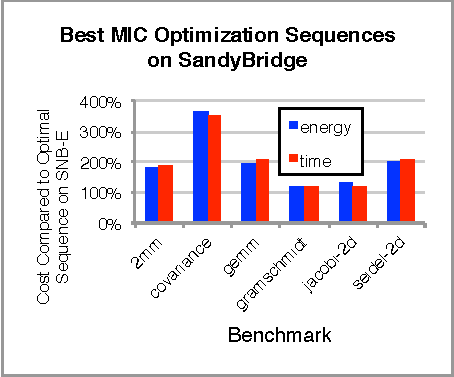
\includegraphics[width=0.45\textwidth]{BestMIConSNB}   
  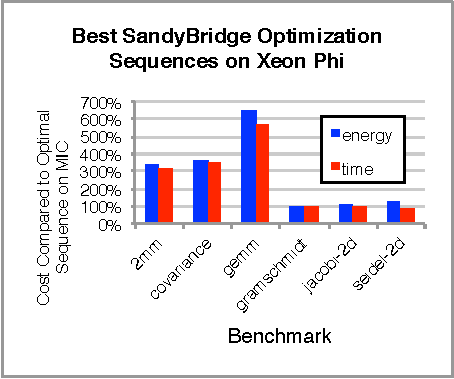
\includegraphics{BestSNBonMIC}
  \label{Sandy}
} 
\subfigure {               
  %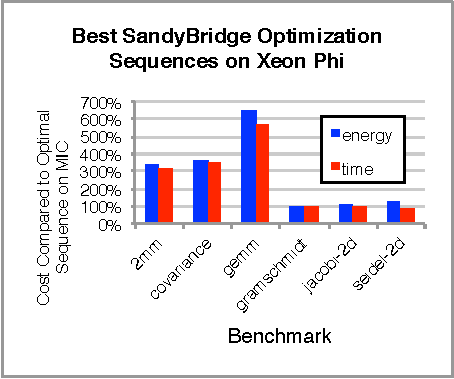
\includegraphics[width=0.45\textwidth]{BestSNBonMIC}
  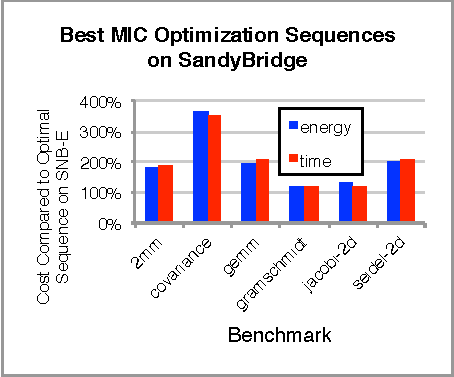
\includegraphics{BestMIConSNB}   
  \label{MIC}
} 
\caption{Cross-Architecture Analysis of Best Optimization Sequences}                   
\label{fig:Brdr2d-TE}                                                   
\end{figure} 

Figure~\ref{Sandy} shows the best optimization sequences of the six benchmarks
chosen from SandyBridge do not perform as good when run on the MIC architecture. 
Comparing with the optimal optimization sequence on the MIC, the SandyBridge
sequences incurred significant increase in execution time and energy consumption
for 2mm, covariance, and gemm. The SandyBridge optimization sequences 
performed as good as the optimal sequence on the MIC for the other three benchmarks. 
Figure~\ref{MIC} compares the time and energy (running on Sandy Bridge) of 
the best optimization sequences chosen from MIC with those of the optimal optimization 
sequences chosen from SandyBridge. 2mm, covariance, gemm, and seidel-2d consumed
from ~200\% to ~350\% more energy and time. 
